\begin{frame}[shrink=60, plain]{Global Standards for Protective Eyewear}
    
    \begin{columns}
        \column{0.5\textwidth}
        \begin{figure}
            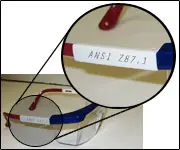
\includegraphics[width=.6\textwidth]{images/Eyewear_pop-out_01-ezgif.com-webp-to-png-converter.png} % Replace with your image path
            \caption{Marker that indicates that the \gls{ped} meets an specifications standard}
        \end{figure}
        
        \textbf{International Standards}
        \begin{itemize}
            \item ISO 12312-1:2013 - Eye and face protection — Sunglasses and related eyewear.
            \item ISO 16321-1:2022 - Eye and face protection for occupational use — General requirements.
            \item ISO 8980-3:2023 - Ophthalmic optics — Uncut finished spectacle lenses.
        \end{itemize}
    
        \textbf{United States}
        \begin{itemize}
            \item ANSI Z87.1-2020 - Occupational and Educational Personal Eye and Face Protection Devices.
            \item OSHA 29 CFR 1910.133 - Standards for eye and face protection in the workplace.
            \item FDA 21 CFR 801.410 - Impact-resistant lenses in eyeglasses and sunglasses.
        \end{itemize}
    
        \textbf{European Union}
        \begin{itemize}
            \item EN 166:2001 - Personal eye-protection specifications.
            \item EN 170:2002 - UV filters for industrial eye protection.
            \item EN 172:1994 - Sunglare filters for industrial use.
        \end{itemize}
    
        \column{0.5\textwidth}
        \textbf{Australia/New Zealand}
        \begin{itemize}
            \item AS/NZS 1337.1:2010 - Eye and face protectors for occupational applications.
            \item AS/NZS 1067.1:2016 - Sunglasses and fashion spectacles.
        \end{itemize}
    
        \textbf{Canada}
        \begin{itemize}
            \item CSA Z94.3-2020 - Eye and face protectors for industrial and other applications.
            \item CAN/CSA-Z94.3.1-16 - Protective eyewear for sports and recreational activities.
        \end{itemize}
    
        \textbf{Japan}
        \begin{itemize}
            \item JIS T 8147:2010 - Eye protection for laser use.
            \item JIS T 8141:2020 - Personal eye-protection equipment.
        \end{itemize}
    
        \textbf{China}
        \begin{itemize}
            \item GB 14866-2006 - National standard for protective eyewear.
            \item GB/T 38120-2019 - General technical requirements for protective eyewear.
        \end{itemize}
    
        \textbf{India}
        \begin{itemize}
            \item IS 5983:1980 - Eye protectors for industrial use.
            \item BIS IS 5983:2018 - Personal eye protection specifications.
        \end{itemize}
    
        \textbf{South Africa}
        \begin{itemize}
            \item SANS 1404:2020 - Eye and face protection.
        \end{itemize}
    
        \textbf{Brazil}
        \begin{itemize}
            \item ABNT NBR 9737:2016 - Eye and face protection for industrial and general use.
        \end{itemize}
    \end{columns}
    \end{frame}
    